\section{实验:用伏特表测电压}\label{sec:8-4}

在这个实验里我们将练习正确使用伏特表。
学生实验最常用的伏特表,是图 \ref{fig:8-12} 甲、乙所示的有三个接线柱、两个量程的伏特表。
在用伏特表测量电压之前,先要仔细观察所用的伏特表,看看它有几个量程,各是多少,
弄清刻度盘上每一个格的数值,并且检查指针是是否对准零刻度。

\begin{figure}[htbp]
    \centering
    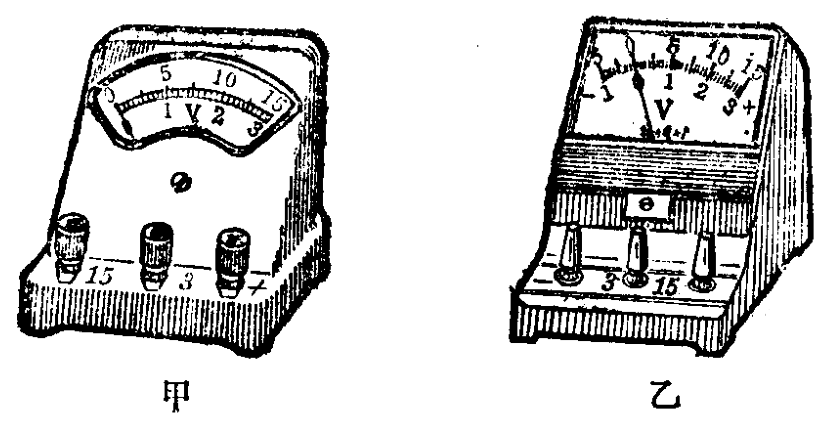
\includegraphics[width=0.7\textwidth]{../pic/czwl2-ch8-12}
    \caption{}\label{fig:8-12}
\end{figure}

在这个实验里我们初次使用伏特表,为了避免接错,每次用伏特表测量之前都要先画好电路图,
在伏特表符号两侧标上代表两个接线柱的 “$+$” “$-$” 号,经检查无误后再照图连接。

首先用伏特表测出每个电池的电压和这几个电池串联成的电池组的电压。
记下测得的值,并且回答:电池组的电压跟串联的各电池的电压之和有什么关系?

然后照图 \ref{fig:8-13} 甲连接串联电路。测出 $L_1$ 两端的电压 $U_1$、
$L_2$ 两端的电压 $U_2$ 以及 $L_1$ 和 $L_2$ 串联后的总电压 $U$。
记下测得的值,并且回答:串联电路两端的总电压跟各部分电路两端的电压之和有什么关系?

\begin{figure}[htbp]
    \centering
    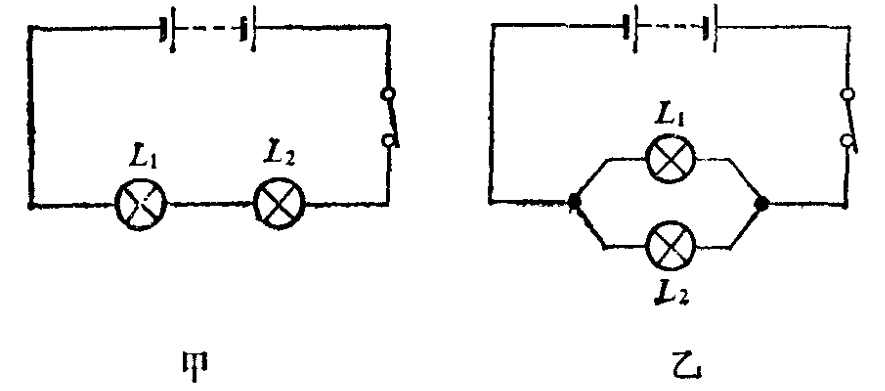
\includegraphics[width=0.7\textwidth]{../pic/czwl2-ch8-13}
    \caption{}\label{fig:8-13}
\end{figure}

最后照图 \ref{fig:8-13} 乙连接并联电路。用伏特表依次测出每个小灯泡两端的电压,
记下测量结果并回答:在并联电路里,各支路两端的电压有什么关系?



\lianxi

(1) 一台晶体管收音机要求电源的电压是 6 伏特。
如果用干电池作电源,需要将几节干电池串联起来?
如果用铅蓄电池作电源,需要几个串联起来?

(2)  在图 \ref{fig:8-14} 中:

\begin{figure}[htbp]
    \centering
    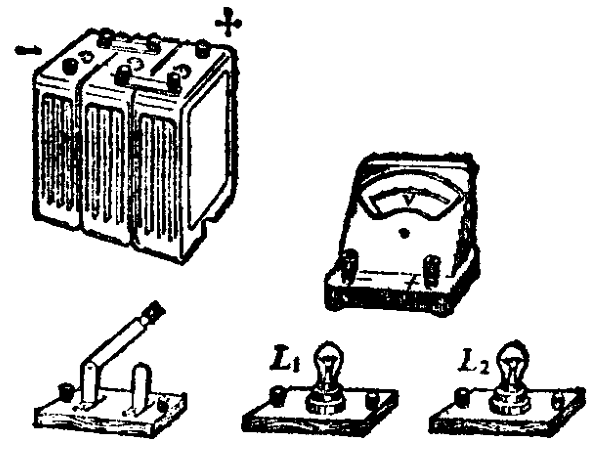
\includegraphics[width=0.5\textwidth]{../pic/czwl2-ch8-14}
    \caption{}\label{fig:8-14}
\end{figure}

\tc{1} 将电灯 $L_1$、$L_2$ 串联起来,用伏特表测电灯 $L_1$ 两端的电压,在图上画出连接方法。

\tc{2} 如果用伏特表测出电灯 $L_1$ 两端的电压是 2 伏特,电灯 $L_1$ 和 $L_2$ 和串联后的总电压是 6 伏特,
那么电灯 $L_2$ 两端的电压是多大?

(3)  画电路图:由电池组(两只电池串联)、电键、小灯泡组成串联电路,
用安培表(要标上 “$+$”、“$-$” 号)测量通过小灯泡的电流强度,
用伏特表(要标上 “$+$”、“$-$” 号)测量小灯泡两端的电压。

(4) 上题中,安培表用的是 0 ~ 0.6 挡,伏特表用的是 0 ~ 15 挡。
各表指针指示位置如图 \ref{fig:8-15} 所示,那么上题中小灯泡里的电流强度和小灯泡两端的电压各是多大?
能换用安培表、伏特表的另一量程来测小灯泡的电流、电压吗?

\begin{figure}[htbp]
    \centering
    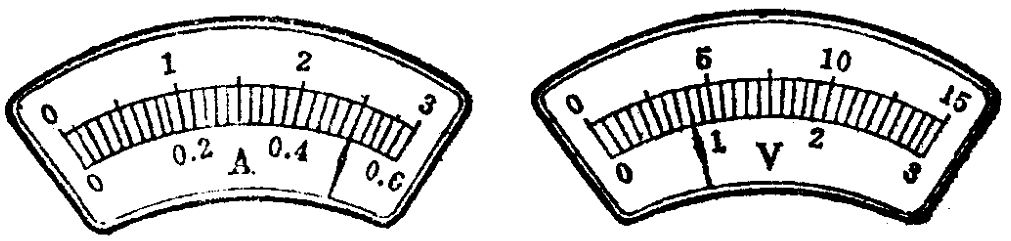
\includegraphics[width=0.7\textwidth]{../pic/czwl2-ch8-15}
    \caption{}\label{fig:8-15}
\end{figure}

(5)  观察一些电器(如普通白炽灯泡、手电筒灯泡、收音机、电视机、录音机、洗衣机、电风扇、电动机等)
铭牌或说明书上标的电压值,并记在作业本上。如果上面还标有电流值,把电流值也记在本上。

